\documentclass[tikz,border=5mm,12pt]{standalone}

\begin{document}
  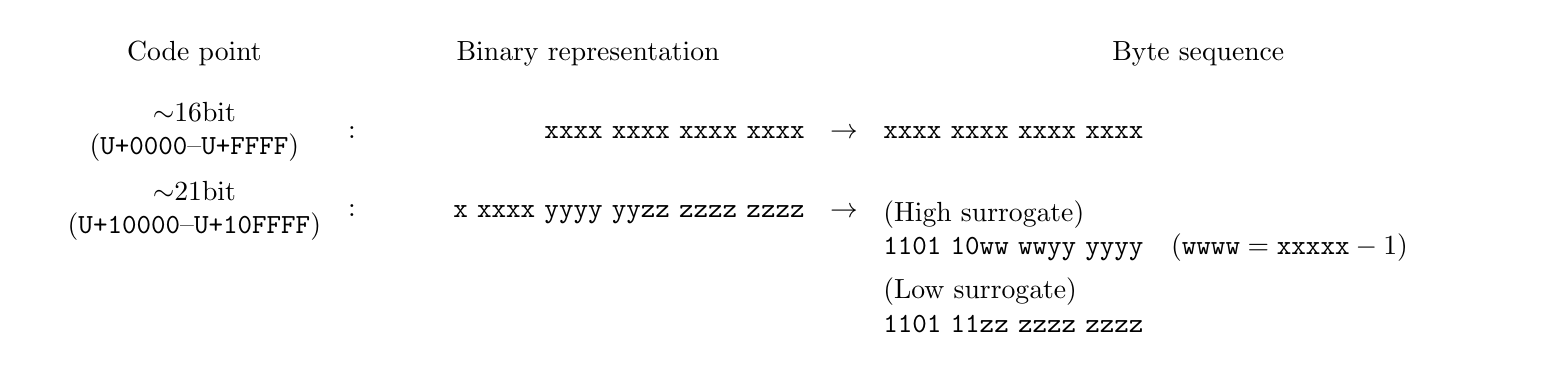
\begin{tikzpicture}
    \node[text width=40mm,align=center] at (0,0) {Code point\strut};
    \node[text centered,text width=40mm] at (0,-10mm) {
      $\sim$16bit \\
      (\texttt{U+0000}--\texttt{U+FFFF})};
    \node[text centered,text width=40mm] at (0,-20mm) {
      $\sim$21bit \\
      (\texttt{U+10000}--\texttt{U+10FFFF})};

    \node at (20mm,-10mm) {:};
    \node at (20mm,-20mm) {:};

    \node[text width=55mm,align=center] at (50mm,0) {Binary representation\strut};
    \node[align=right,text width=55mm] at (50mm,-10mm) {\texttt{xxxx xxxx xxxx xxxx}\strut};
    \node[align=right,text width=55mm] at (50mm,-20mm) {\texttt{x xxxx yyyy yyzz zzzz zzzz}\strut};

    \node at (82.5mm,-10mm) {$\rightarrow$\strut};
    \node at (82.5mm,-20mm) {$\rightarrow$\strut};

    \node[text width=80mm,align=center] at (127.5mm,0) {Byte sequence};
    \node[align=left,text width=80mm] at (127.5mm,-10mm) {\texttt{xxxx xxxx xxxx xxxx}\strut};
    \node[align=left,text width=80mm,text depth=0mm,minimum height=35mm] at (127.5mm,-20mm) {(High surrogate)\\
      \texttt{1101 10ww wwyy yyyy}\strut \quad$(\texttt{wwww} = \texttt{xxxxx}-1)$\\
      \vspace{4pt}
      (Low surrogate) \\
      \texttt{1101 11zz zzzz zzzz}\strut};
  \end{tikzpicture}
\end{document}
